\subsection{Nativer Mobile Client}

Dieses Kapitel beschreibt das Konzept für einen nativen iOS Client zur Bedienung von Praxisruf.
Es wird Entwurf und Funktionsweise der notwendigen Ansichten der Benutzeroberfläche beschrieben.
Weiter wird definiert, wie die aus dem Vorgängerprojekt zu migrierenden Funktionen in eine native iOS Applikation integriert werden können.
Dies beinhaltet insbesondere Anbindung der API des Cloudservice und Firebase Cloud Messaging.
Die Integration von Gegensprechanlage und Sprachsynthese wird nur im Rahmen des Entwurfs der Benutzeroberfläche beschrieben.
Eine detaillierte Beschreibung der Konzepte für diese Features folgt in den Kapiteln 7.3 und 7.4.


\subsubsection{Benutzeroberfläche}

Die Ansichten zur Anmeldung und Zimmerauswahl werden analog zum bestehenden Mobile Client umgesetzt.
Die Loginseite beinhaltet einen kurzen Willkommenstext und ein Logo für Praxisruf.
Darunter findet sich ein einfaches Formular zur Eingabe von Benutzername und Passwort, sowie ein Button zur Bestätigung.

\begin{figure}[h]
    \centering
    \begin{minipage}[b]{0.4\textwidth}
        \fbox{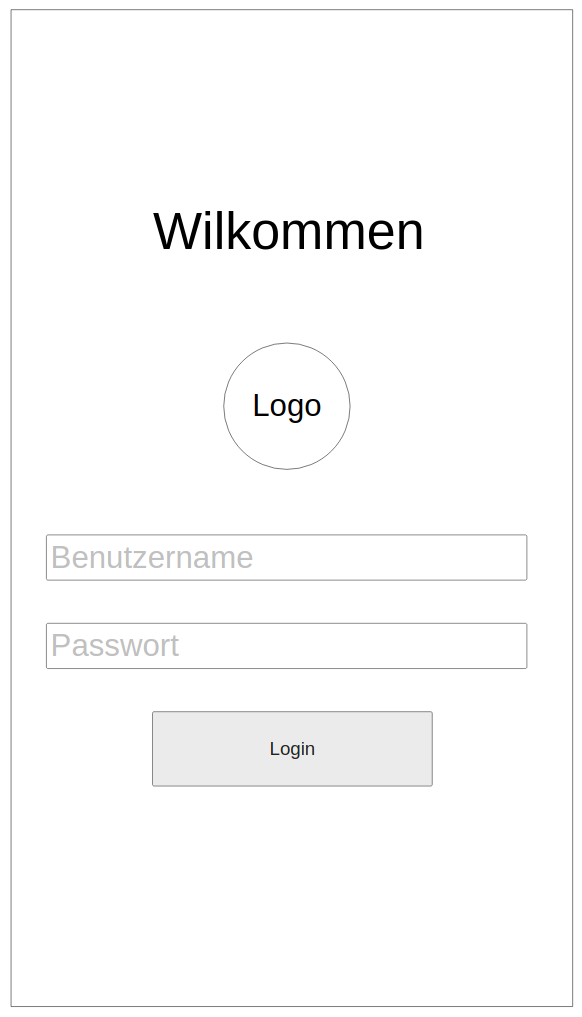
\includegraphics[width=\textwidth]{/home/joshua/FHNW/dev/IP6/IP6_Bachelorarbeit_Bericht_Cloudbasiertes_Praxisrufsystem/src/graphics/mockups/mockup_login}}
        \caption{Mockup Login}
    \end{minipage}
    \hfill
    \begin{minipage}[b]{0.4\textwidth}
        \fbox{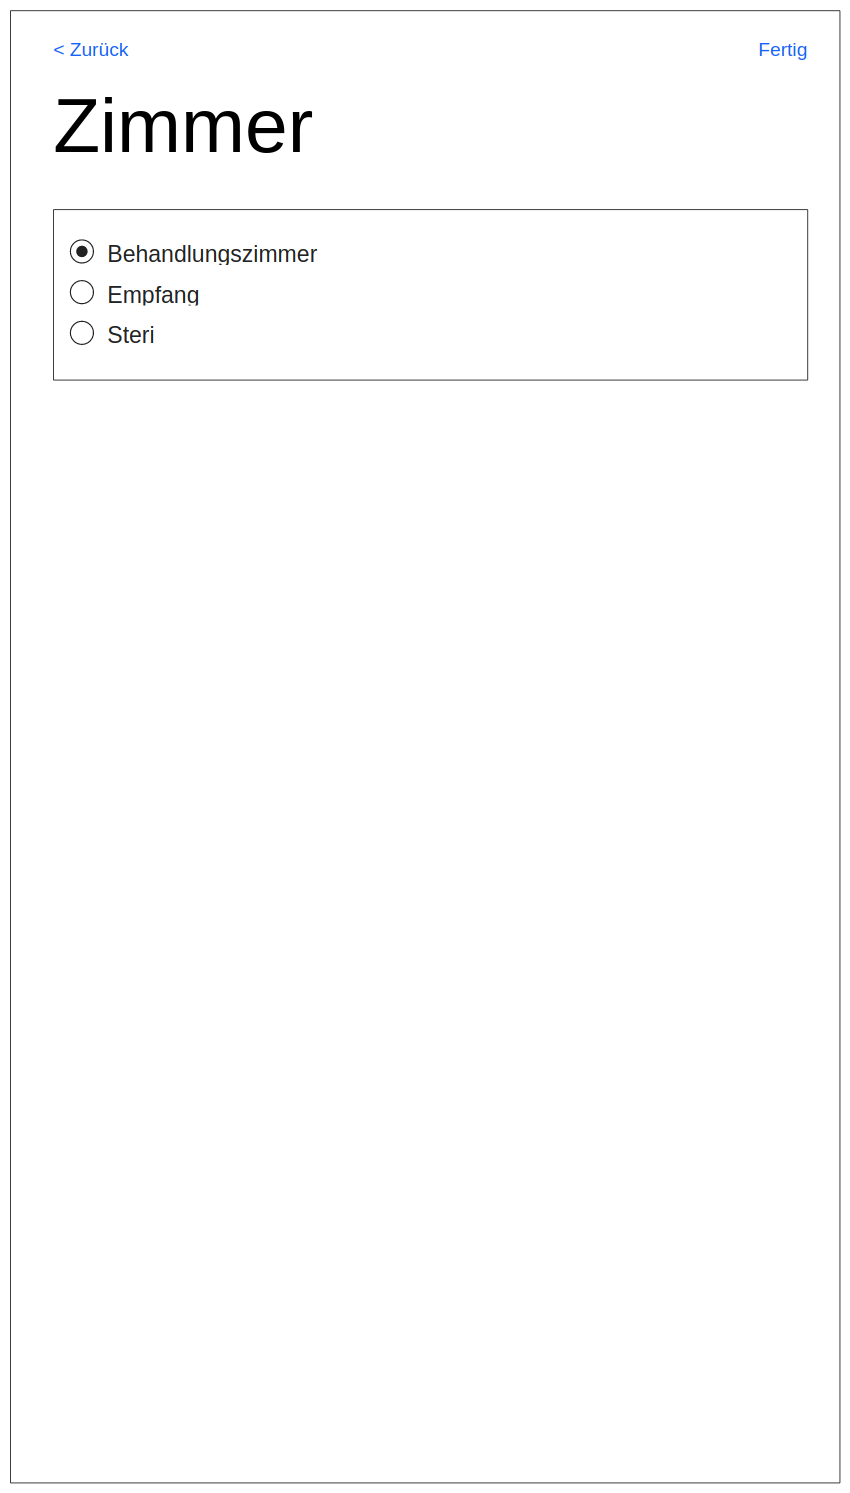
\includegraphics[width=\textwidth]{/home/joshua/FHNW/dev/IP6/IP6_Bachelorarbeit_Bericht_Cloudbasiertes_Praxisrufsystem/src/graphics/mockups/mockup_clientselect}}
        \caption{Mockup Zimmerwahl}
    \end{minipage}\label{fig:Mockups-Login-ClientSelection}
\end{figure}

Nach dem Eingeben der Anmeldedaten werden Praxismitarbeitende aufgefordert, die gewünschte Konfiguration auszuwählen.
Die Ansicht besteht aus einem Seitentitel und einer Liste zur Auswahl der gewünschten Konfiguration.
In der Auswahl sind alle Zimmer zu sehen, welche dem Benutzer zur Verfügung stehen.
Diese Konfigurationen müssen vor der Anmeldung im Admin UI erfasst und dem Benutzer zugewiesen werden.
In der Kopfzeile sind die Schaltflächen ''Zurück'' und ''Fertig'' zu sehen.
Die Schaltfläche ''Zurück'', bricht die Anmeldung ab und führt zurück zur Eingabe der Logindaten.
Die Schaltfläche ''Fertig'' bestätigt die Auswahl und leitet zur Hauptansicht weiter.
Wird bestätigt, ohne dass ein Zimmer angewählt ist, wird dem Benutzer eine Fehlermeldung angezeigt und nicht zur Hauptansicht weitergeleitet.

Die Hauptansicht der Applikation gliedert sich in die Bereiche Home, Inbox und Einstellungen.
Zwischen den drei Bereichen kann über eine Leiste am unteren Ende des Bildschirms navigiert werden.
Die Ansicht Home zeigt dem Benutzer die Buttons, über welche er Benachrichtigungen versenden und Anrufe in der Gegensprechanlage starten kann.
Wird ein Anruf gestartet, wird die Ansicht für aktive Anrufe angezeigt.
Diese zeigt dem Benutzer den Titel des gestarteten Anrufs, sowie eine Liste aller Teilnehmer zusammen mit dem Verbindungsstatus jedes Teilnehmers.
Der Titel des Anrufes entspricht dem Anzeigetext des verwendeten Buttons für ausgehende Anrufe und dem Namen des Anrufers für empfangene Anrufe.
Neben den Anrufinformationen zeigt die Ansicht für aktive Anrufe drei Buttons.
Über diese können Mikrofon und Lautsprecher des eigenen Gerätes stumm geschaltet werden.
Weiter kann der Anruf über einen roten Button am rechten Rand beendet werden.
Nach einem beendeten Anruf wird automatisch zu der zuvor angezeigten Ansicht navigiert.

\begin{figure}[h]
    \centering
    \begin{minipage}[b]{0.4\textwidth}
        \fbox{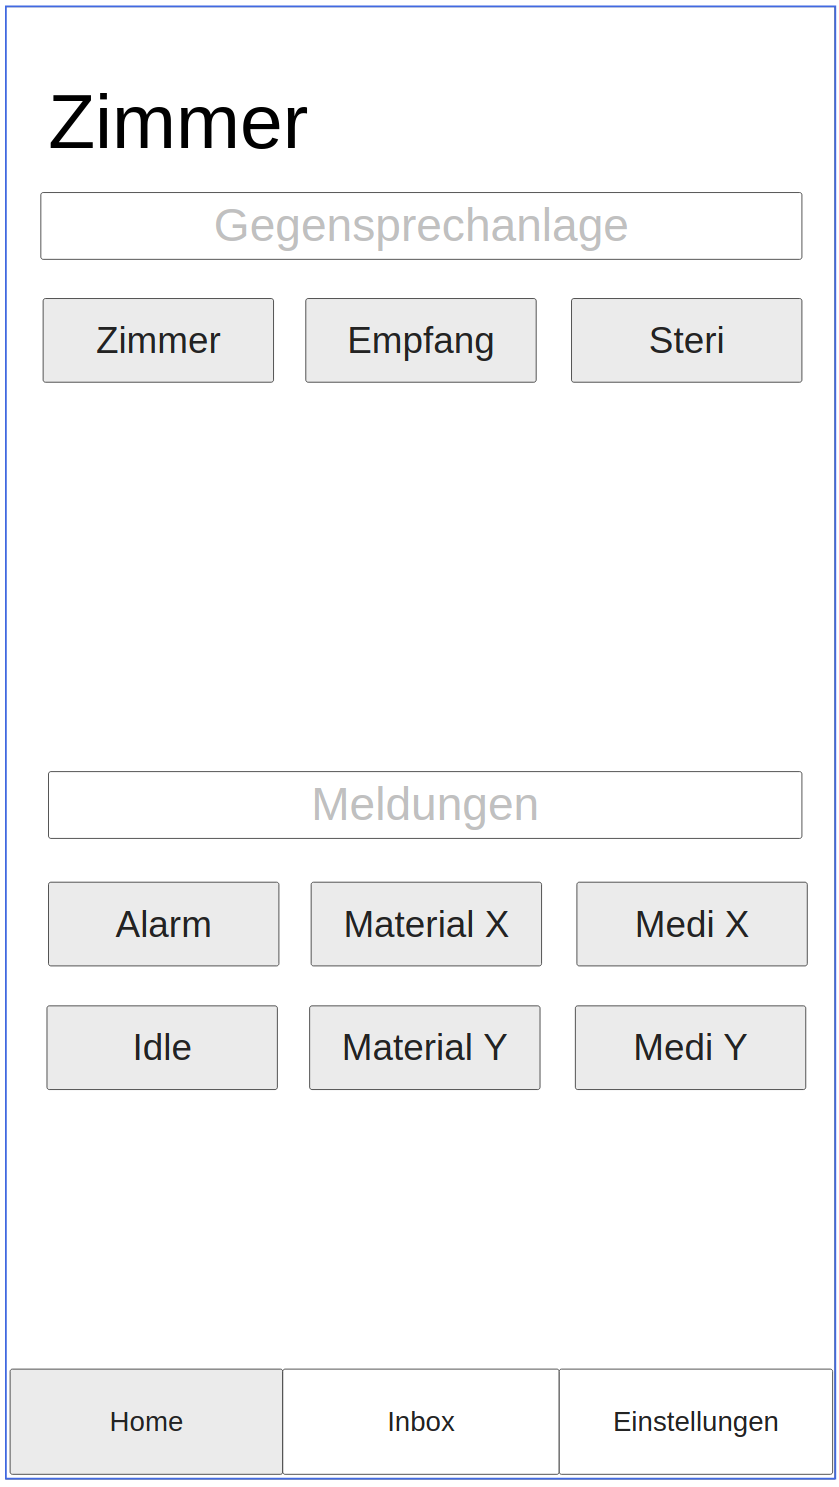
\includegraphics[width=\textwidth]{/home/joshua/FHNW/dev/IP6/IP6_Bachelorarbeit_Bericht_Cloudbasiertes_Praxisrufsystem/src/graphics/mockups/mockup_intercom}}
        \caption{Mockup Home}
    \end{minipage}
    \hfill
    \begin{minipage}[b]{0.4\textwidth}
        \fbox{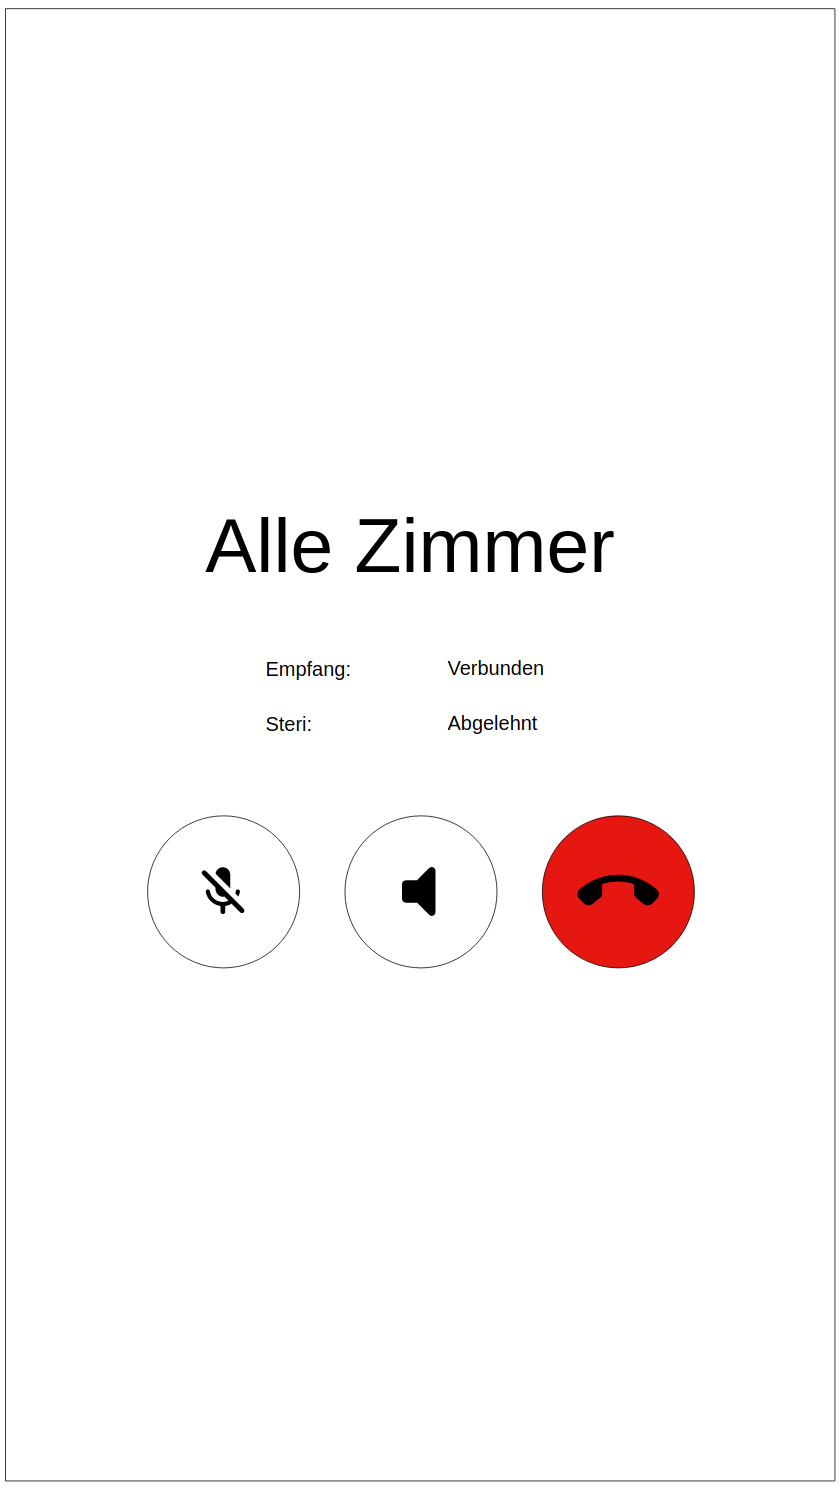
\includegraphics[width=\textwidth]{/home/joshua/FHNW/dev/IP6/IP6_Bachelorarbeit_Bericht_Cloudbasiertes_Praxisrufsystem/src/graphics/mockups/mockup_call}}
        \caption{Mockup Aktiver Anruf}
    \end{minipage}\label{fig:Mockups-Home-ActiveCall}
\end{figure}

Der Bereich Inbox zeigt eine Liste der empfangenen Benachrichtigungen sowie der empfangenen und verpassten Anrufe.
Für alle Elemente in der Inbox wird der Name des Senders als Überschrift angezeigt.
Darunter werden weitere Detailinformationen beschrieben.
Für Benachrichtigungen beinhaltet dies den Textinhalt der Benachrichtigungen.
Bei Anrufen beschrieben ob, es sich um einen empfangenen, verpassten oder abgelehnten Anruf handelt.
Einträge für Benachrichtigungen sowie verpasste und abgelehnte Anrufe müssen durch eine Wischgeste quittiert werden.
Die Funktionsweise der Quittierung wird aus dem bestehenden Mobile Client übernommen.
Quittierte Meldungen werden aus der Inbox entfernt und nicht mehr angezeigt.
Ein Quittieren von Meldungen und Anrufen passiert ausschliesslich lokal in der iOS Applikation.
Der Empfänger wird nicht über die Quittierung informiert~\cite{ip5}.

Es muss sichergestellt werden, dass verpasste Benachrichtigungen und Anrufe nicht übersehen werden.
Dazu wird im Abstand von 60 Sekunden geprüft, ob unquittierte Benachrichtigungen oder Anrufe in der Inbox vorhanden sind.
Ist dies der Fall, wird ein Erinnerungston abgespielt und eine Benachrichtigung angezeigt.
Dieser Mechanismus wird in Kapitel 7.2.4 weiter beschrieben.

\begin{figure}[h]
    \centering
    \begin{minipage}[b]{0.4\textwidth}
        \fbox{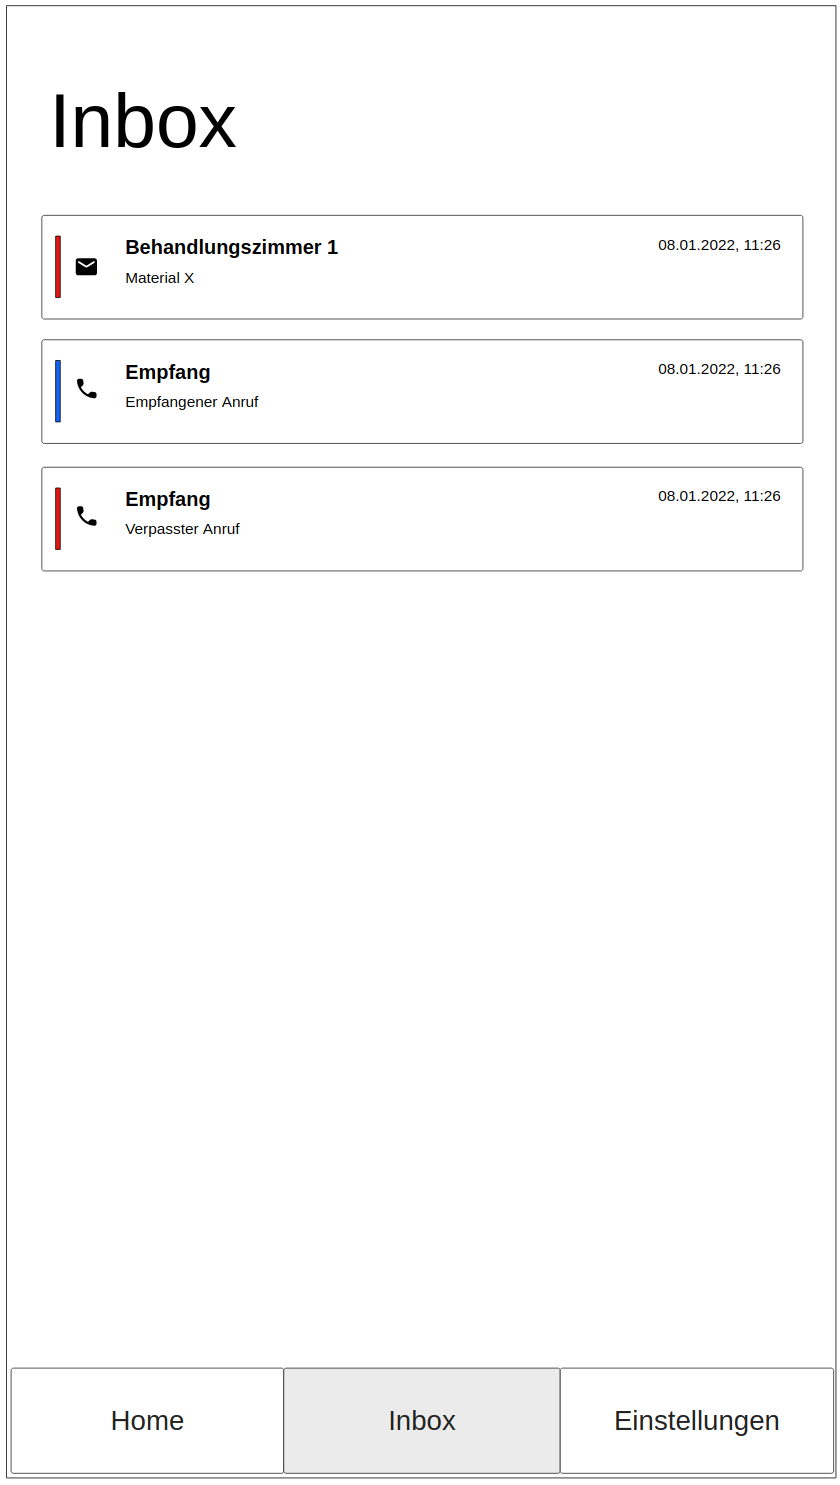
\includegraphics[width=\textwidth]{/home/joshua/FHNW/dev/IP6/IP6_Bachelorarbeit_Bericht_Cloudbasiertes_Praxisrufsystem/src/graphics/mockups/mockup_inbox}}
        \caption{Mockup Inbox}
    \end{minipage}
    \hfill
    \begin{minipage}[b]{0.4\textwidth}
        \fbox{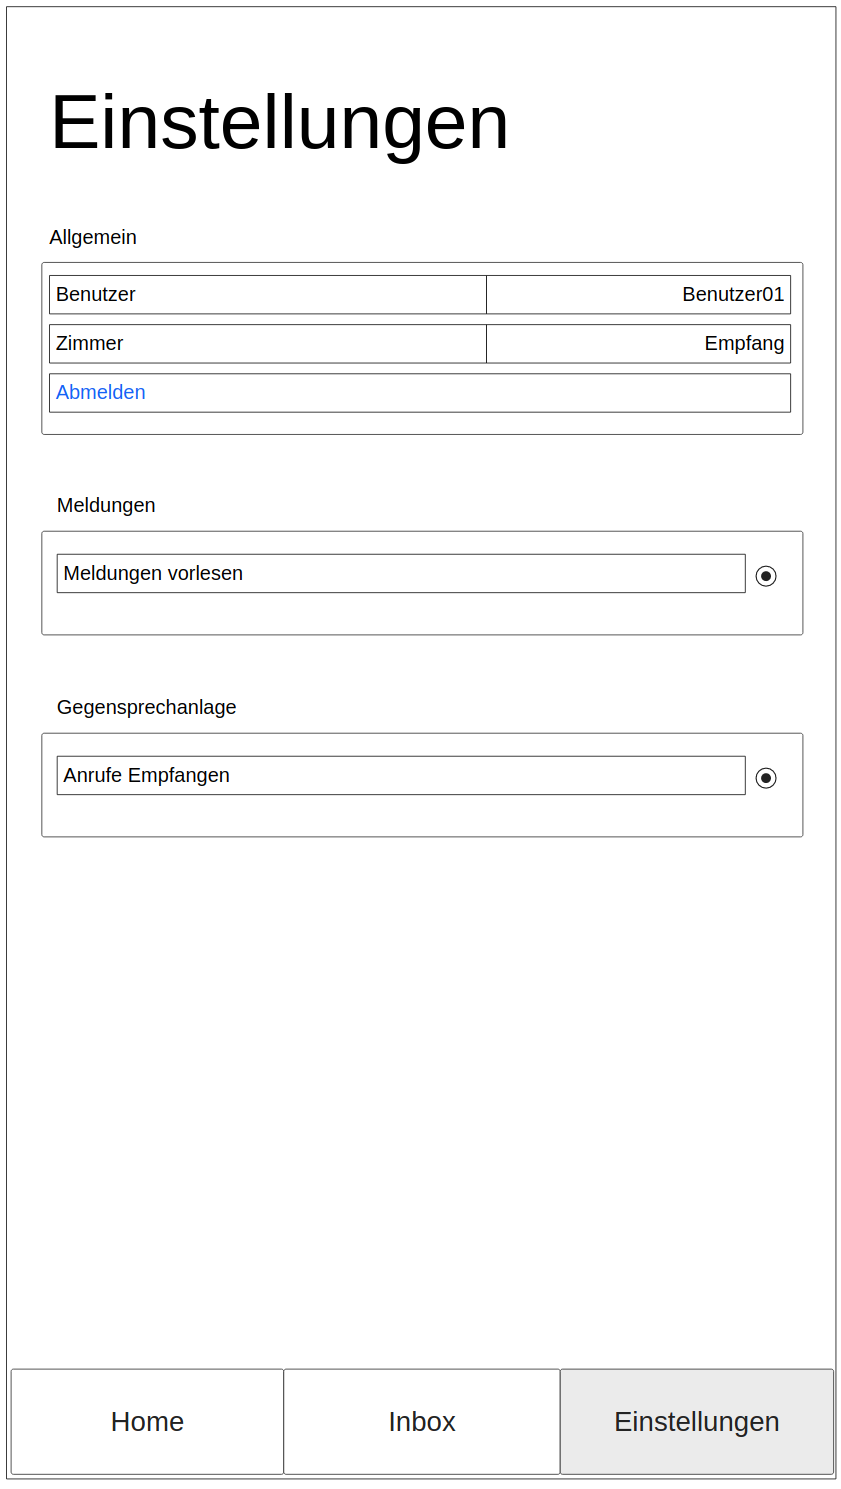
\includegraphics[width=\textwidth]{/home/joshua/FHNW/dev/IP6/IP6_Bachelorarbeit_Bericht_Cloudbasiertes_Praxisrufsystem/src/graphics/mockups/mockup_settings}}
        \caption{Mockup Einstellungen}
    \end{minipage}\label{fig:Mockups-Inbox-Settings}
\end{figure}

Abbildung 7.8 zeigt den Bereich Einstellungen.
Der Bereich Einstellungen zeigt den aktuellen Benutzernamen und die gewählte Konfiguration.
Über die Schaltfläche Abmelden, können sich Praxismitarbeitende aus der Applikation abmelden.
Die Schaltfläche Benachrichtigungen vorlesen ist standardmässig aktiviert.
Wird die Option deaktiviert, werden Benachrichtigungen nie vorgelesen.
Die Schaltfläche Anrufe empfangen ist ebenfalls standardmässig aktiviert.
Wird diese Option deaktiviert, werden alle empfangenen Anrufe automatisch abgelehnt und stattdessen eine Benachrichtigung angezeigt.
Ausgehende Anrufe können auch getätigt werden, wenn diese Option aktiviert ist.

\subsubsection{Anbindung Cloudservice API}

Der Mobile Client muss an die API des Cloudservices angebunden werden.
Es wird eine Anbindung an die Domäne Configuration zur Anmeldung und Auswahl des gewünschten Zimmers und an die Domäne Notification zum Versenden von Benachrichtigungen benötigt.
Die Schnittstellen dieser Domänen stehen als Http Endpunkte zur Verfügung.
In diesem Unterkapitel wird beschrieben, wie Http-Anfragen an die Cloudservice API in den nativen iOS Client integriert werden.
Das Abrufen von Sprachdaten und die Anbindung an die Signaling Instanz werden in den Kapiteln 7.3 und 7.4 beschrieben.

Die Basisbibliothek für iOS Entwicklung bietet die Klasse URLSession, über welche Netzwerkaufrufe getätigt werden können.
Über URLSession.shared steht eine Standard-Instanz zur Verfügung, über welche Netzwerkanfragen verarbeitet werden können~\cite{ios_urlsession}.
Die Klasse UrlRequest ermöglicht es, Http-Request für eine URL mit Header und Body zu erstellen~\cite{ios_urlrequest}.
Um die Integration dieser Klassen in die Applikation zu vereinfachen, wird ein zentraler Service mit dem Namen PraxisrufApi erstellt.
Dieser kapselt das Erstellen, Befüllen und Absetzten der nötigen UrlRequest Instanzen.
Er bietet öffentliche Methoden für die Http Verben Get, Post und Delete an.
Über diese können Http-Requests mit der jeweiligen Methode abgesetzt werden.
Zur Darstellung von Fehlern wird die Enum PraxisrufApiError erstellt.
Diese definiert Fehlerkategorien und wird von PraxisrufApi verwendet, um Aufrufern das Fehlschlagen einer Anfrage mitzuteilen.
Das Klassendiagramm in Abbildung 7.9 zeigt den Aufbau des Service PraxisrufApi\@.

\begin{figure}[h]
    \centering
    \begin{minipage}[b]{0.8\textwidth}
        \fbox{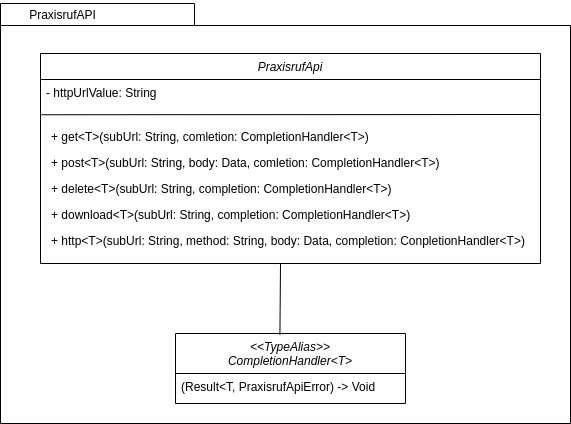
\includegraphics[width=\textwidth]{graphics/diagramms/Class_PraxisrufAPI_V01}}
        \caption{Klassendiagramm PraxisrufApi}
    \end{minipage}
\end{figure}

Die Basis-URL für Http-Anfragen wird in der Konfiguration der iOS Applikation definiert.
Der PraxisrufApi Service lädt diese und verwendet sie für alle Abfragen, die abgesetzt werden.
Alle öffentlichen Methoden von PraxisrufApi nehmen einen Parameter ''subUrl'' als String entgegen.
Dieser String wird der Basis-URL angehängt.
Die Methoden Post nimmt zudem einen optionalen Parameter von Typ Data entgegen.
Dieser definiert den Inhalt des Request Bodies.
Mit diesen Informationen kann der Http Request erstellt und versendet werden.

Sämtliche öffentlichen Methoden des PraxisrufApi Service nehmen weiter einen Parameter mit dem Namen completion entgegen.
Dabei handelt es sich um eine Funktion, welche beim Erfolg oder Fehlschlagen der Http-Anfragen ausgeführt wird.
Als Parameter dieser Funktion wird immer der Typ Result$<$T, PraxisrufApiError$>$ verwendet.
Bei Result handelt es sich um einen Wrapper Typen welcher entweder das Resultat einer Abfrage oder ein Fehlerobjekt beinhaltet~\cite{ios_result}.
Im Fehlerfall wird das Result mit einem PraxisrufApiError Objekt erstellt.
Im Erfolgsfall wird es mit den Daten aus dem Body der Http-Antwort befüllt.
Zur Darstellung dieser Daten wird der generische Typ T verwendet.
Der Typ wird vom Aufrufer von PraxisrufApi definiert und kann grundsätzlich beliebig sein.
Er muss aber das Protokoll Decodable aus der iOS Standardbibliothek implementieren.
Decodable Instanzen können von einer JSON-String-Repräsentation in ein Swift-Objekt konvertiert werden~\cite{ios_decodable}.
So kann das Resultat im Erfolgsfall aus der Response generiert und an, dass Callback übergeben werden.
Dadurch kann die Konvertierung generisch in im PraxisurfApi-Service behandelt werden.

Anhand des Inhalts der Result-Instanz kann geprüft werden, ob die Anfrage erfolgreich war.
Das Resultat kann entsprechend verarbeitet werden.
Diese Prüfung und Verarbeitung findet innerhalb der completion-Funktion statt.
Dieser Ansatz ermöglicht es im PraxisrufApi-Service ausschliesslich Http-Anfragen zu senden und die entsprechenden Antworten entgegenzunehmen.
Der Api Service behandelt damit ausschliesslich die technische Anbindung an die API des Cloudservice.
Er muss keine fachliche Logik implementieren und kann generisch für alle Anwendungen wiederverwendet werden.

Requests die über den PraxisrufApi-Service erstellt werden, werden automatisch authentisiert.
Dazu lädt der Service die hinterlegten Credentials aus dem KeyStore von iOS.
Das Token wird verwendet, um einen entsprechenden Authorization-Header zu generieren.
Der generierte Authorization Header wird der Http-Anfrage angefügt.
Ist kein Token vorhanden, wird keine Anfrage abgesetzt.
Es wird direkt die completion-Funktion mit dem Fehler PraxisrufApiError.invalidCredential aufgerufen.

Mit dieser Lösung steht ein Service zur Verfügung, über welchen Http-Anfragen einfach in eine iOS App integriert werden können.
Dank der generischen Methoden im PraxisrufApi-Service können neue Calls einfach hinzugefügt werden, ohne das Boilerplate-Code wiederholt werden muss.
Durch die completion-Funktionen kann die fachliche Verarbeitung von Http-Anfragen vom Aufrufer definiert werden.

Um die Verwendung der Cloudservice API weiter zu vereinfachen, wird der PraxisrufApi Service um sprechende Methoden für die nötigen Abfragen erweitert.
Dazu wird pro Domäne eine Extension-Klasse erstellt.
Diese fügt Methoden mit sprechenden Namen für die angesprochene Funktionalität hinzu und kapseln die Verwendung der Get, Post und Delete Methoden.

Der PraxisrufApi-Service ermöglicht es Abfragen an die Cloudservice API abzusetzen.
Die Resultate dieser Abfragen müssen in der Benutzeroberfläche angezeigt werden können.
Es wird pro Domäne ein weiterer Service geschrieben, welche den Aufruf des API Services kapselt.
Dieser Service bietet Methoden, über welche der PraxisrufApi Service angesprochen werden kann.
View-Komponenten können diese Services nutzen, um durch Benutzereingaben ausgelöste Anfragen an die Cloudservice Api zu senden.
Resultate und Fehler aus Anfragen an den Cloudservice werden in diesen Services als Instanzvariablen gehalten.
Die View-Komponenten können lesend auf diese Variablen zugreifen, um die entsprechenden Resultate oder Fehler anzuzeigen.

\subsubsection{Anbindung Messaging Service}

Um Benachrichtigungen empfangen zu können, muss Firebase Cloud Messaging an die native iOS Applikation angebunden werden.
Firebase bietet eine Bibliothek mit welcher Firebase Cloud Messaging in iOS Clients integriert werden kann~\cite{firebase_ios}.
Diese Integration kann allerdings nicht mit dem Mitteln von SwiftUI implementiert werden.
Dies liegt daran, dass für das Empfangen von Benachrichtigungen und das Anzeigen von Push-Benachrichtigungen Integration mit dem Benachrichtigungszenter des Betriebssystem notwendig ist.
Diese Integration kann bis heute nur über AppDelegates umgesetzt werden.
SwiftUI Applikationen können oft ohne AppDelegates implementiert werden.
Sobald aber Integration mit dem Betriebssystem notwendig ist, müssen AppDelegates verwendet werden.
Dazu können AppDelegates bei der Initialisierung der Applikation registriert werden.

Zur Anbindung von Firebase Cloud Messaging wird dementsprechend ein AppDelegate implementiert.
Die Logik des Delegates wird dabei auf das minimal Nötige reduziert.
Der AppDelegate selbst ist für die direkte Kommunikation mit Firebase verantwortlich und muss empfangene Daten an Betriebssystem und SwiftUI Applikation übergeben.
Fachliche Logik wird nicht im AppDelegate, sondern in der SwiftUI Applikation ausgeführt.
Dies ermöglicht es die Anbindung des Messaging Service im AppDelegate zu kapseln.
Sollte Firebase Cloud Messaging in Zukunft durch einen anderen Anbieter ersetzt werden, muss damit ausschliesslich die Logik im AppDelegate angepasst werden.
Diese Trennung stellt sicher, dass die Fachlogik vollständig mit SwiftUI implementiert werden kann.
Der AppDelegate beinhaltet lediglich die Teile, welche aus technischen Gründen nicht mit SwiftUI umgesetzt werden können.

Um Benachrichtigungen von Firebase Cloud Messaging empfangen zu können, muss der AppDelegate folgende Funktionalität umsetzen.
Beim Start der Applikation muss sich der Mobile Client beim Messaging Service registrieren.
Nach der Registrierung wird für den Mobile Client ein Token generiert, welches den Client eindeutig beim Messaging Service identifiziert.
Der AppDelegate muss, darauf reagieren und das erneuerte Token an die Applikation übergeben.

Für die Verarbeitung von Benachrichtigungen muss der AppDelegate Benachrichtigungen im Vordergrund empfangen und dem Betriebssystem zur Anzeige übergeben.
Die Informationen aus der empfangenen Benachrichtigung müssen anschliessend an die Applikation übergeben werden.
Benachrichtigungen, die im Hintergrund empfangen werden, müssen an das Betriebssystem übergeben und angezeigt werden.
Sobald die Applikation wieder in den Vordergrund tritt, müssen die Daten an die Applikation zur weiteren Verarbeitung übergeben werden.

\subsubsection{Benachrichtigungen prüfen}

Der bestehende Mobile Client prüft in regelmässigen Abständen, ob ungelesene Benachrichtigungen in der Inbox vorhanden sind.
Wenn ungelesene Benachrichtigungen gefunden werden, wird ein Benachrichtigungston abgespielt.
Im Mobile Client der Vorgängerlösung findet diese Prüfung nur statt, wenn die Applikation in Vordergrund aktiv ist.
Diese Funktion wird in der nativen iOS Applikation übernommen.

Für die Umsetzung der Erinnerungsfunktion werden zwei Services definiert.
Erstens wird eine Inbox erstellt, welche eine Liste der aktuellen Benachrichtigungen führt.
Zweitens wird ein InboxReminderService implementiert.
Dieser prüft den Inhalt der Inbox und sucht nach unquittierten Elementen, welche älter als eine Minute sind.
Werden solche Elemente gefunden, wird eine Benachrichtigung angezeigt und ein Benachrichtigungston abgespielt.
Die regelmässige Prüfung der Inbox wird mit der Timer-Klasse der iOS Standardbibliothek umgesetzt.
Über diese ist es möglich auf einer View in regelmässigen Abständen Events auszulösen~\cite{ios_timer}.
Ein solcher Timer wird auf der Hauptansicht für angemeldete Benutzer registriert.
Der Timer löst alle 60 Sekunden die Prüfung des InboxReminderService aus.

Die Prüfung von Benachrichtigungen im Hintergrund wird im Rahmen dieses Projektes nicht umgesetzt.
Für künftige Erweiterungen ist es möglich diese Funktion zu implementieren.
Um dies zu ermöglichen, müssen Benachrichtigungen auf dem Gerät persistiert werden.
So stehen die Daten auch zur Verfügung, wenn die Applikation nicht gestartet ist.
Weiter muss ein Hintergrundtask implementiert und registriert werden~\cite{ios_bgtaskscheduler}, welcher die persistierten Daten lädt und die darauf die Prüfung des InboxReminderService ausführt.

\subsubsection{Security}

In einem Praxisrufsystem muss die sichere Übertragung von Daten gewährleistet sein.
Die dazu definierten Konzepte werden aus dem Vorgängerprojekt übernommen.

Alle Daten zwischen den Services müssen über verschlüsselte Verbindungen ausgetauscht werden.
HTTP Anfragen CloudService API erfolgen ausschliesslich über HTTPS\@.
Alle Anfragen an die API des Cloudservice müssen zudem mit einem Json Web Token (JWT) authentifiziert sein.
Praxismitarbeitende werden durch den Cloudservice mittels Basic Authentication authentifiziert.
Bei der Anmeldung mit Benutzername und Passwort liefert der Cloudservice ein JWT, welches vom Client für weitere Anfragen verwendet wird.
Sowohl die Credentials für die Basic Authentication als auch das JWT Token werden durch die iOS Applikation im Keystore des Betriebssystems gespeichert~\cite{ip5}.
Das Token wird regelmässig erneuert, indem die Basic Authentication mit den gespeicherten Credentials wiederholt wird.
Der Ablauf für Authentifizierung wird damit unverändert aus dem Vorgängerprojekt übernommen.

\clearpage

\subsubsection{Servicemodell}

Dieses Kapitel gibt einen Überblick zu den Services welche in der nativen iOS Applikation beinhaltet werden.
Abbildung 7.10 zeigt das vollständige Modell der implementierten Services.
Diese Darstellung beinhaltet die Services, welche in den Kapiteln 7.2 bis 7.4 beschrieben werden.
View- und Model-Komponenten werden hier nicht dargestellt.

\begin{figure}[h]
    \centering
    \begin{minipage}[b]{1\textwidth}
        \fbox{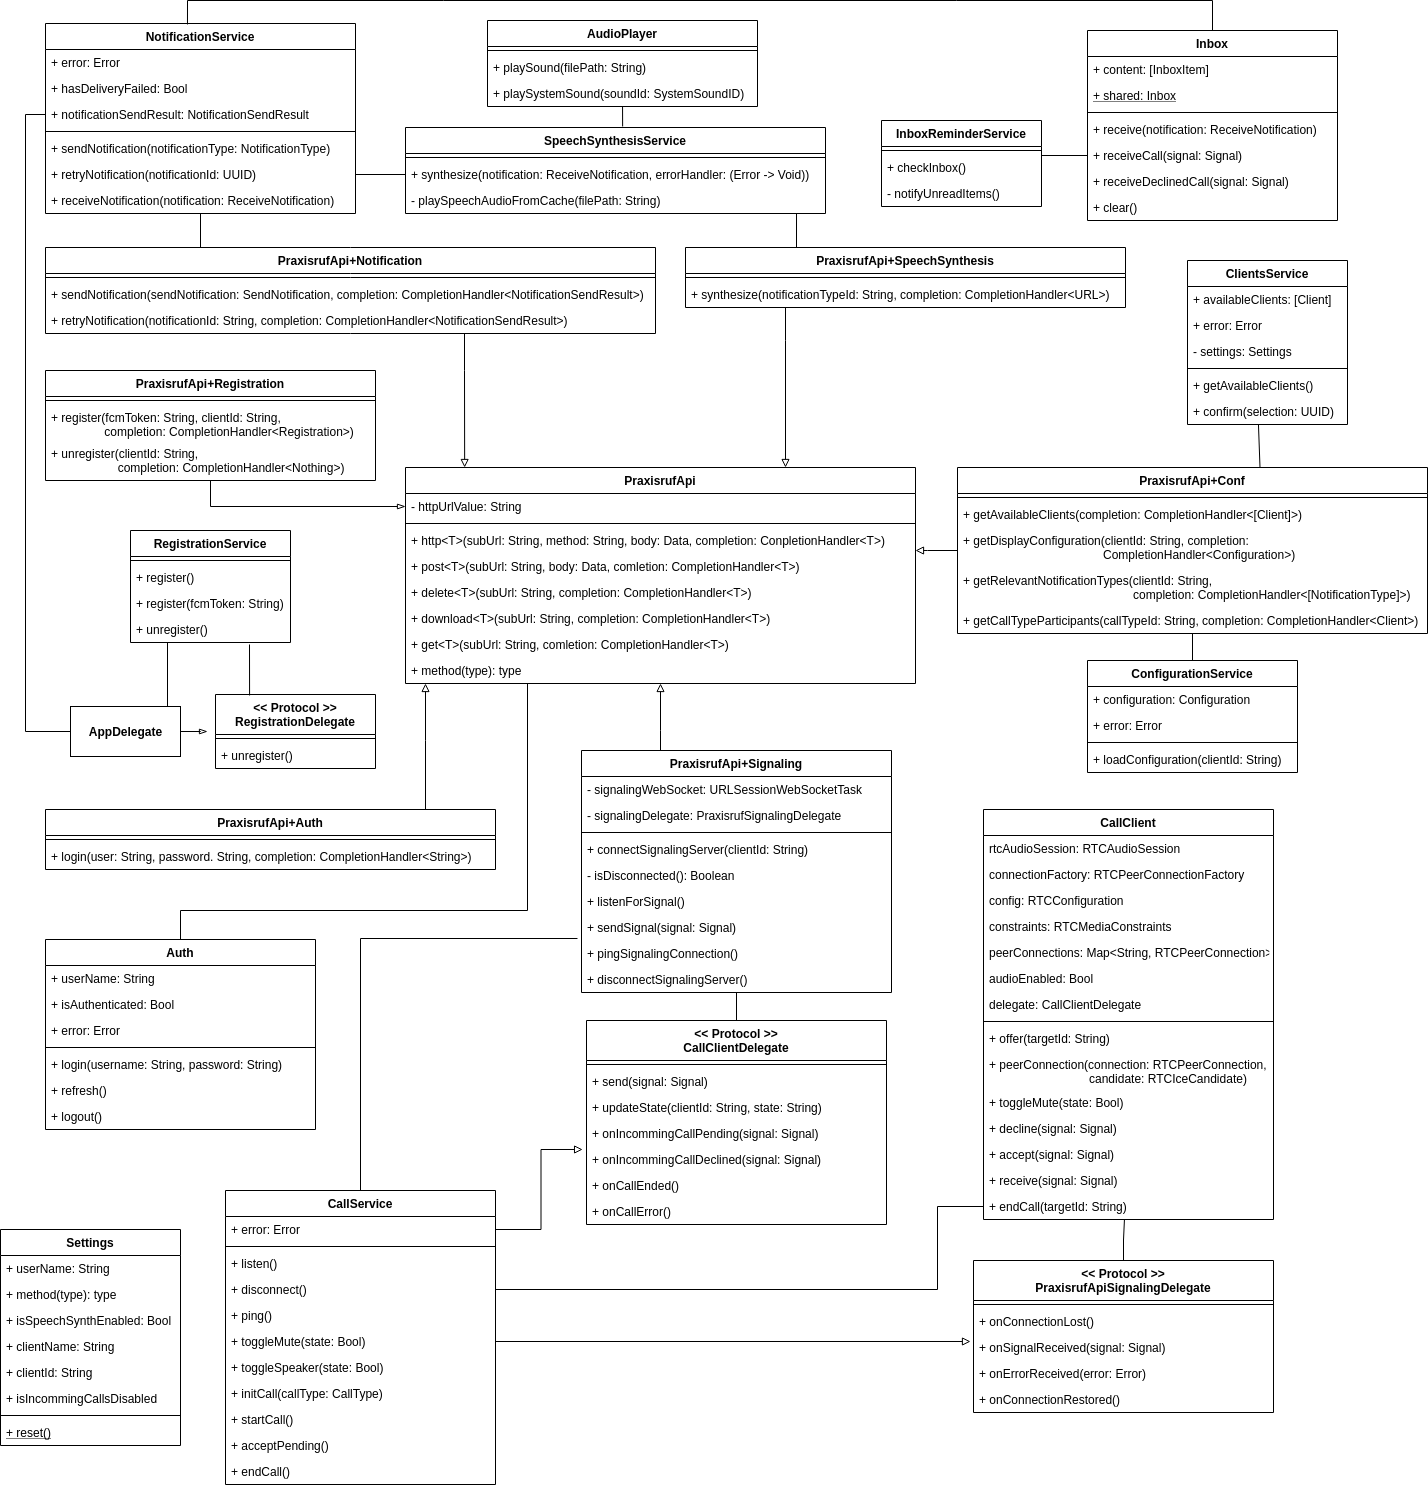
\includegraphics[width=\textwidth]{/home/joshua/FHNW/dev/IP6/IP6_Bachelorarbeit_Bericht_Cloudbasiertes_Praxisrufsystem/src/graphics/diagramms/Class_Mobile_Client_Draft_V02}}
        \caption{Klassendiagramm Modul SpeechSynthesis}
    \end{minipage}
\end{figure}

Die Klasse Settings wird verwendet um die Konfiguration des Benutzers zu verwalten.
Sie bietet Getter und Setter für alle Properties.
Nach dem setzten eines Wertes, wird dieser über die Komponente UserData aus der iOS Standardbibliothek persistiert.
Die Verwendungen der Settings-Klasse sind in Abbildung 7.10 nicht dargestellt, um die Übersichtlichkeit zu wahren.

\clearpage
